%!TEX root = main.tex

\subsection{Motivations}

\begin{itemize}
	\item multiple alignments are most often based on pairwise alignments;
	\item a new sequence x may be only distantly and locally related to each sequence in a known family (biological question): all pairwise alignments between x and each family members will look poor. We need to model \textbf{statistical features} shared by the family members;
	\item computing the alignment between x and a probabilistic model of the family may be much \textbf{more efficient computationally}.
\end{itemize}

\subsection{Position specific scoring matrices}

\begin{figure}[H]
	\centering
	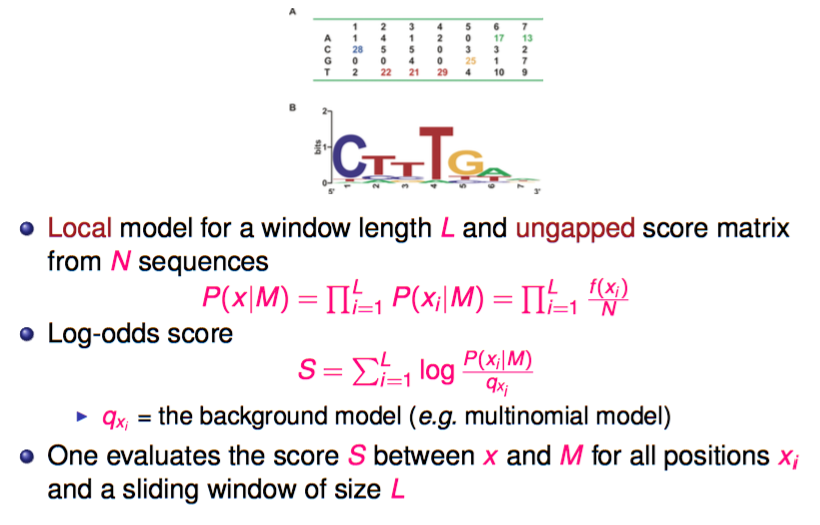
\includegraphics[scale=0.5]{images/37_pssm.png}
	\caption{PSSMs are very simple HMMs. $P(x_i|M)$ are emission probabilities on match state. Transition probabilities are equal to 1. But we need to account for possible gap and avoid a prescribed window length.}
\end{figure}

\begin{figure}[H]
	\centering
	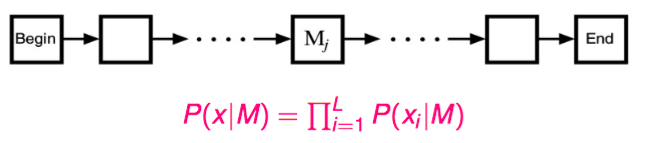
\includegraphics[scale=0.6]{images/40_pssm.png}
\end{figure}

\subsection{Full profile HMMs}

\subsubsection{Adding insert states}

\begin{figure}[H]
	\centering
	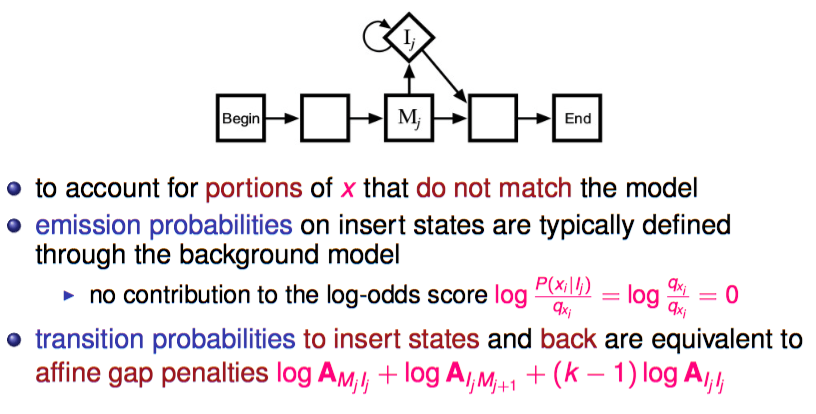
\includegraphics[scale=0.5]{images/38_insert.png}
\end{figure}

\subsubsection{Adding delete states}

\begin{figure}[H]
	\centering
	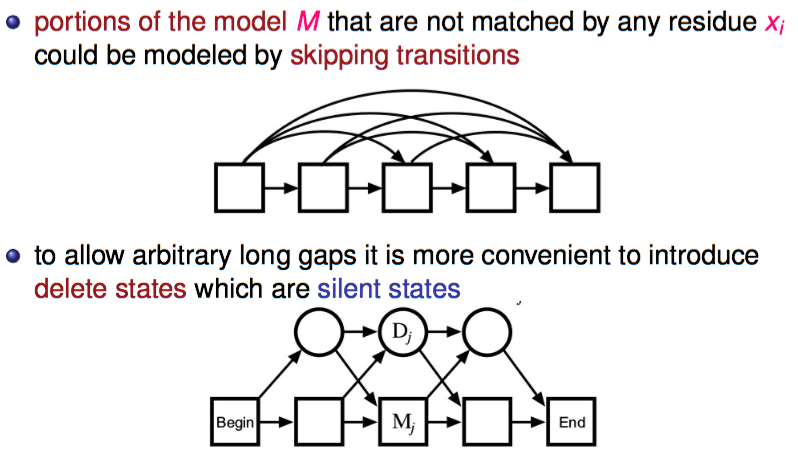
\includegraphics[scale=0.5]{images/39_delete.png}
	\caption{More convenient because less transitions.}
\end{figure}

\subsubsection{A full profile HMM}

\begin{figure}[H]
	\centering
	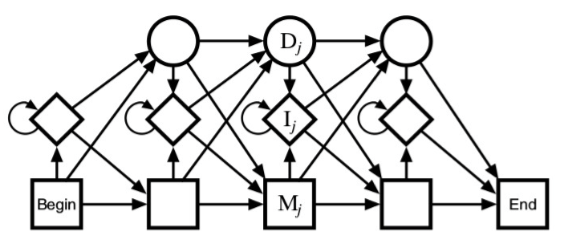
\includegraphics[scale=0.6]{images/41_phmm.png}
	\caption{Parameters are: value of the probabilities and length. Begin, End and D states are silent.}
\end{figure}

\subsubsection{Deriving a pHMM from a multiple alignement (Supervised)}


\begin{figure}[H]
	\centering
	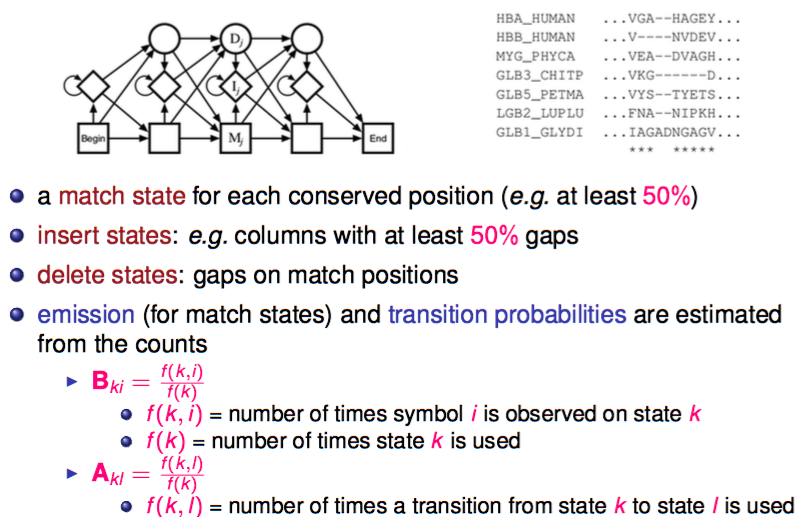
\includegraphics[scale=0.5]{images/42_deriving.png}
\end{figure}

But the initial multiple alignement could have some probabilities equal to zero: we need \textbf{smoothing}.

\begin{figure}[htp]
	\centering
	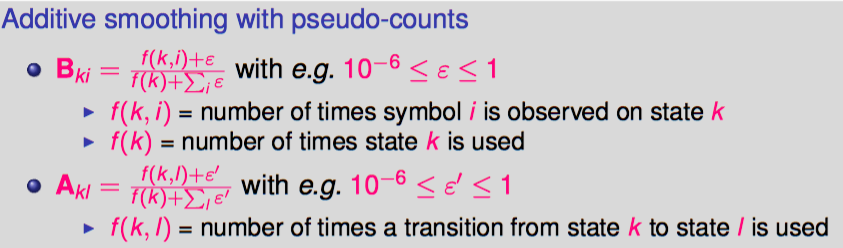
\includegraphics[scale=0.5]{images/43_smoothing.png}
\end{figure}

\subsubsection{Unsupervised learning}

No need for an initial multiple alignment (only unaligned sequences).

\begin{figure}[htp]
	\centering
	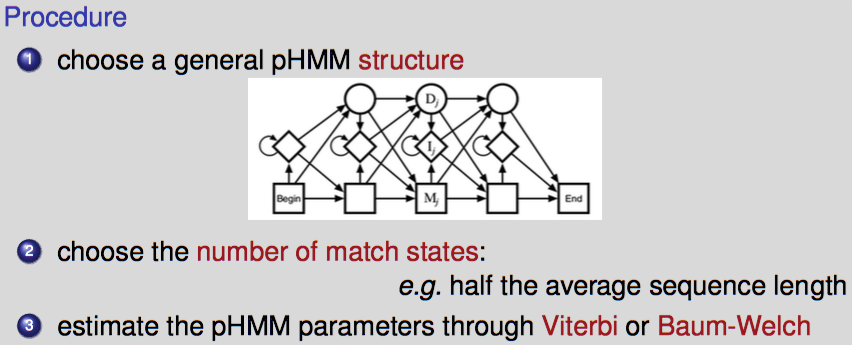
\includegraphics[scale=0.5]{images/44_unsupervised.png}
\end{figure}

\subsubsection{Matching a sequence to a pHMM a.k.a. viterbi recurrence}


\begin{figure}[H]
	\centering
	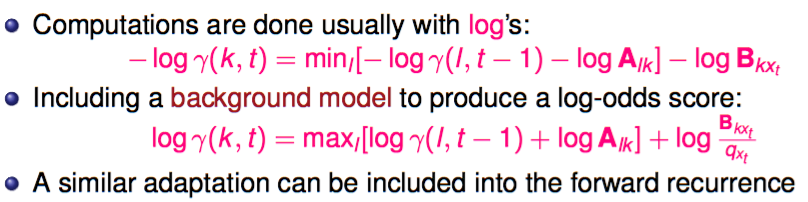
\includegraphics[scale=0.5]{images/45_viterbi.png}
\end{figure}

\newpage

\subsubsection{For non-global alignments}


\begin{figure}[H]
\begin{adjustwidth}{-2cm}{}
\centering
\begin{minipage}{.47\linewidth}
  \centering
  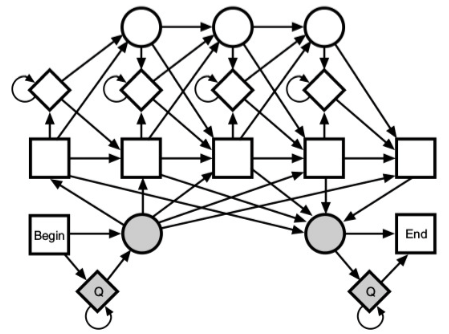
\includegraphics[scale=0.5]{images/46_nglobal.png}
  \caption{Local alignment (S-W style). Non-conserved fragments are modeled through flanking insert states using the backgroud emission probabilities $q_a$. Their loop have high probabilities. Flanking delete states allow for starting or ending the profile at any point and reduce number of transitions.}
\end{minipage}%
\hspace{0.5cm}
\begin{minipage}{.47\linewidth}
  \centering
  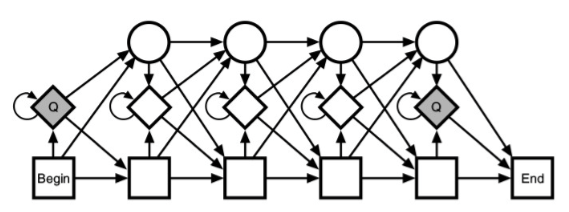
\includegraphics[scale=0.5]{images/47_nglobal.png}
  \caption{Set all the transition probabilities from the left flanking state to different start points. Force the match on the compelte profile.}
\end{minipage}
\end{adjustwidth}
\end{figure}

\begin{figure}[htp]
	\centering
	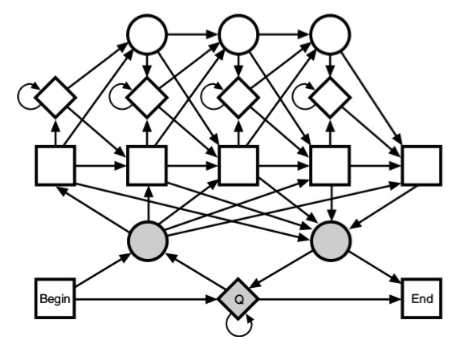
\includegraphics[scale=0.5]{images/48_nglobal.png}
	\caption{Allow repeated matches to subsections of the profile.}
\end{figure}


